\documentclass[
    % a4paper,
    ebook,
    11pt,
    % twoside,
    oneside,
    onecolumn,
    openright,
    final
    % draft
]{memoir}

\usepackage[]{geometry}
% \usepackage[final]{microtype}
\usepackage{indentfirst}

\usepackage{amsmath}
\usepackage{amsfonts}
\usepackage{amssymb}
\numberwithin{equation}{section}

\usepackage{physics}
\usepackage{tensor}

\usepackage{graphicx}

\usepackage{natbib}

\usepackage{kotex}
\usepackage{lipsum}

\usepackage{hyperref}
\hypersetup{%
    unicode=true,
    colorlinks=false
}

\usepackage{xcolor}

\begin{document}

\begin{titlingpage}
    \title{\HUGE\textbf{Notes on Electrodynamics}}
    \author{\Large\textbf{Nanaki}}
    \date{\Large{\today}}

    \pagenumbering{Alph}
    \maketitle
    \begin{center}
        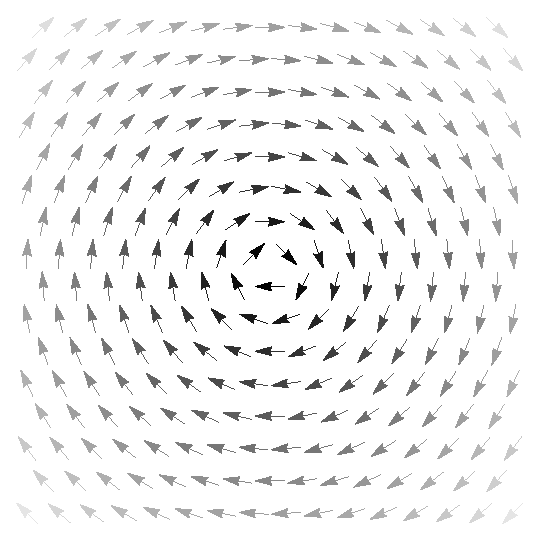
\includegraphics[width=0.8\textwidth]{figures/cover.pdf}
    \end{center}
\end{titlingpage}

\frontmatter

\tableofcontents
% \clearpage

\mainmatter

% === Introduction ===
% \part{Introduction}
% \chapter{Classical Electrodynamics and Special Relativity}


% === Special Relativiy ===
\part{The Special Theory of Relativity}

\chapter{The Principle of Relativity}

\chapter{Physical Interpretation}

\chapter{Minkowski Geometry}

\chapter{Relativistic Mechanics}

% === Classical Electrodynamics ===
\part{Fundamental Electrodynamics}

\chapter[Charges in EM Fields]{Charges in Electromagnetic Fields}
\section{Elementary Particles in the Theory of Relativity}
\label{sec:05a-01a}

상대론적 역학을 논하기 전에 고전역학에서 배운 내용을 생각해보자. 고전역학에서는 입자들의 상호작용(interaction)을 기술하기 위해서 장(field)을 사용한다. 좀 더 구체적으로 말하자면 입자가 주위에 장을 생성하면 다른 모든 입자가 이 장에 영향을 받아서 힘을 받게 된다. 고전역학에서 장은 입자들의 상호작용이라는 물리적인 현상을 설명하는 방식의 하나이다.
그런데 상대성 이론에서는 상호작용의 전파 속도가 유한하므로 상황이 근본적으로 다르다. 입자에 작용하는 힘은 더는 힘이 작용하는 순간 입자가 어디에 있는지만으로 결정되지 않는다. 한 입자의 위치가 변하면 그 변화는 특정 시간 간격이 지나간 후에 다른 입자에 영향을 준다. 이는 장 자체가 물리적으로 실제\footnote{동역학을 갖고 있다.}한다는 것을 의미한다. 우리는 더는 서로 멀리 떨어져 있는 입자들의 직접적인 상호작용에 대해서 말할 수 없다. 상호작용은 공간적으로 인접한 지점 사이에서 한순간에 발생할 수 있다. 따라서 우리는 한 입자와 장의 상호작용 그리고 장과 두 번째 입자의 후속 상호작용에 대해 말해야 한다.

입자와 전자기장의 상호작용을 고려하기 전에 상대론적 역학에서 입자란 무엇인지에 대해 생각해보자.
고전역학에서는 어떤 조건에서도 모양과 부피가 변하지 않는\footnote{물체 안의 임의의 두 점 사이의 거리가 일정한} 물체를 도입했다. 이를 강체(rigid body)라 부른다. 그러나 상대성 이론은 강체가 존재하지 않는다고 말한다. 증명은 간단하다. 일단 강체가 존재한다고 가정하자. 이 강체에 외력이 작용한다면 강체의 모든 지점은 힘이 가해지는 지점과 동시에 움직여야 한다. 그렇지 않으면 변형된다. 그러나 상대성 이론에 따르면 특점 지점에 가해지는 힘은 유한한 속도로 다른 지점에 전달되어 모든 지점이 동시에 움직일 수 없다. 따라서 귀류법에 따라 강체는 존재하지 않는다.

위의 논의에서 우리는 상대론적 역학\footnote{Classical (non-quantum) relativistic mechanics}에서는 기본 입자(elementary particle)는 반드시 점으로 다루어야 한다는 것을 알 수 있다.

\section{Four-Potential of a Field}


\section{Equations of Motion of a Charge in a Field}
\label{sec:05a-03a}



\chapter[The EM Field Equations]{The Electromagnetic Field Equations}

\chapter[Constant EM Fields]{Constant Electromagnetic Fields}

% === Electrodynamics of Continuous Media
\part{Electrodynamics of Continuous Media}

\chapter{Electrostatics of Conductors}

\chapter{Electrostatics of Dielectrics}

\chapter{Steady Current}

\chapter{Magnetostatics}

\chapter{Ferromagnetism and Antiferromagnetism}

\chapter{Quasi-Static Electromagnetic Field}

% === Electromagnetic Waves ===
\part{Electromagnetic Waves}

\chapter{Electromagnetic Waves}

\chapter{The Propagation of Electromagnetic Waves}

\chapter{The Field of Moving Charges}
% 2-VIII 8-XIV

\chapter{Radiation of Electromagnetic Waves}

\chapter{Scattering of Electromagnetic Waves}

\chapter{Diffraction of Electromagnetic Waves}
% 2-59 2-60 2-61

% === Appendices ===
\appendix
\part{Appendix}

\chapter{Mathematical Tools}
% Multipole Expansion

\backmatter

\end{document}
